\subsection{Model design}

The actor and critic models architecture is shown in figure \ref{fig:model}. 
The input is separated in two categories: static and dynamic data. 
Static data is infomation that doesn't change as nodes are being placed, such as: computation graph and tile memory constraint.
Device state, node to be placed and placed node latencies are dynamic data that changes during placement.

Tile memory variables need to be placed in a tile so that operation can use that variable. This memory constraint is captured as 
memory dependency array. Tile memory constraints are incorporated into nodes in the computation graph. The computation graph 
has each node representing an instruction. The node features are tile memory dependencies. A Graph Neural Network (GNN) is 
used to process node dependencies and create an embedding for each node. An attention module is applied to the embedding matrix 
to select which dependency nodes are relevant to the current node to be placed. The dynamic data is fed into a MLP model to 
create another embedding to represent current state. The two embeddings are combined and fed into another MLP model to 
create actions. Invalid actions are masked before being sent to the reward function. Masking was shown to be effective in RL setting \cite{Shengyi_mask}.

\begin{figure}[h]
  \centering
  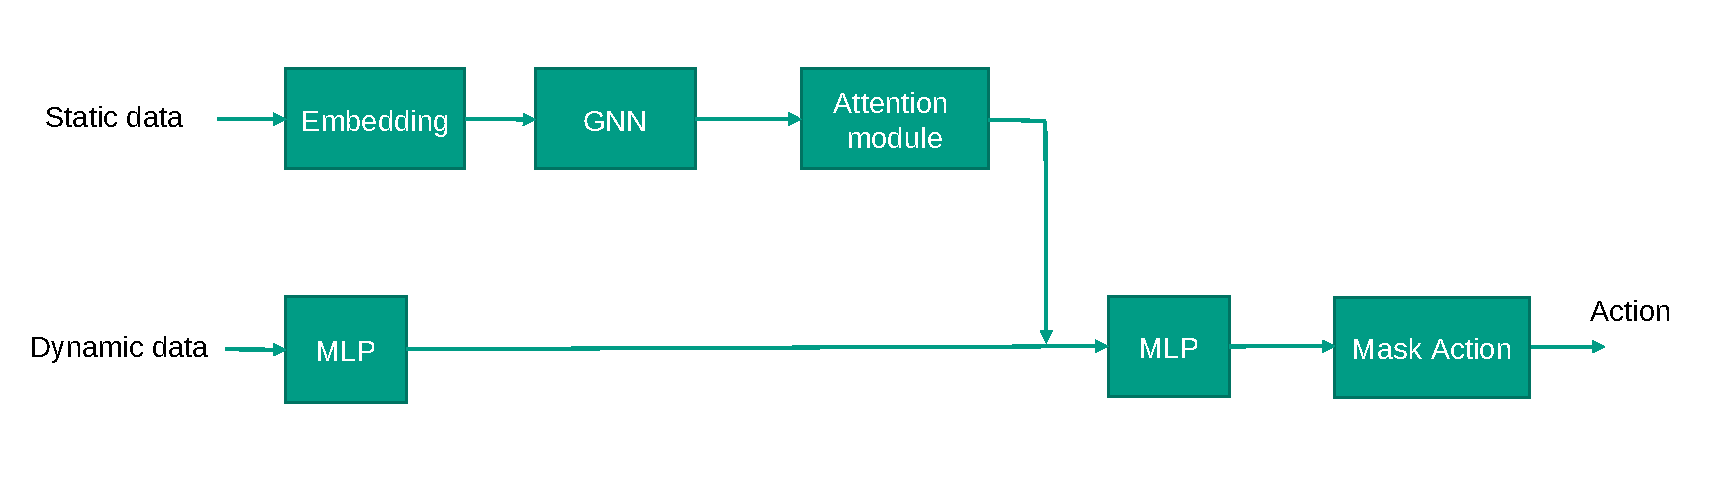
\includegraphics[width=\linewidth]{fig/model.pdf}
  \caption{Actor and critic model architecture. GNN is used to process the computation graph (static data). 
  Attention module gives importance to relevant nodes. The embedding created from dynamic data is combined with static data embedding. 
  A final MLP model is used to generate actions. Actions are masked to ensure only valid actions are produced. }
  \label{fig:model}
\end{figure}

